\chapter{Betriebsaufgaben im Stromnetz der TWS Netz GmbH}
\label{cha:Betriebsaufgaben}

\section{Kontrollen und Untersuchungen gefundener Schäden im Stromnetz}

Unter Betrieb versteht man das Betreiben von vorhandener Anlagen, letztlich die Aufrechterhaltung der Versorgung. 
Betriebsaufgaben im Bereich der Stromversorgung haben in Form von Kontrollen vorbeugenden Charakter. Sie setzen sich fort in der Untersuchung gefundener 
oder gemeldeter Schäden mit rechtzeitiger Bekanntgabe erforderlicher Sperrungen, der Errichtung von Umgangsleitungen, dem Stellen von Notversorgungen, 
Abstellungen, Umstellungen und ähnlichem.
\\
Allgemeine Betriebsaufgaben sind hierbei die Überprüfung vorhandener Anlagen auf einwandfreien, betriebssicheren Zustand. Neben von Dritten gemeldeten Schäden
und Mängel sind es diese allgemeine Betriebsaufgaben, die zu Instandsetzungaufgaben führen. Spezielle Betriebsaufgaben sind Aufgaben, die im Zusammenhang 
mit Neubau, Instandsetzungs- oder Fremdaufträgen anfallen. Das Stromnetz ist aufgeteilt in vier verschiedene Spannungsebenen: 
\begin{itemize}
    \item[-] Höchstspannung: Sie dient zur Übertragung von Strom über große Distanzen und wird mit 380 kV betrieben. Durch die hohe Spannung sinken die 
    Leistungsverluste bei der Übertragung über große Distanzen. Dieses Netz wird genutzt, um den Strom von Kraftwerken aus in ganz Deutschland zu verteilen.
    \item[-] Hochspannung: Dieses Netz wird genutzt, um den Strom regional zu Verteilen und Umspannwerke in größeren Städten mit Strom zu versorgen. 
    In Baden-Württemberg ist dieser Betreiber die Netze BW, welcher die lokalen Umspannwerke versorgt und dort den Strom von 110 kV auf 20 kV transferiert.
    \clearpage
    \item[-] Mittelspannung: Das Mittelspannungsnetz wird mit 20 kV betrieben und wird verwendet, um den Strom mit geringeren Leistungsverlusten zu den 
    Umspannstationen zu übertragen. Es wird hauptsächlich für kleinere Strecken genutzt und dient zur Versorgung von ländlichen Regionen oder Stadtteilen.
    \item[-] Niederspannung: Dieses Netz wird mit 0,4 kV betrieben und dient zur Versorgung von Firmen und privaten Immobilien. Es wird ausschließlich über 
    geringe Distanzen genutzt und wird durch eine hohe Anzahl an Umspannstationen möglichst kurzgehalten, da die Leistungsverluste sehr hoch sind bei großen
    Strecken.
\end{itemize}
Das Niederspannungs- und Mittelspannungsnetz gehört zum Aufgabenbereich der TWS Netz GmbH und wird durch Sie verwaltet. \autocite{Schwab.2012} 
\\
Die Aufgaben im Niederspannungsnetz betreffen überwiegend die Kabelverteilerschränke und beziehen sich auf die Sichtkontrolle von intakten Sicherungen, 
angesammeltem Verunreinigungen und sicherheitsrelevanten Beschädigungen. Des Weiteren müssen Holz oder Stahlmasten, an denen Freileitungen hängen in 
regelmäßigen Abständen kontrolliert und dokumentiert werden, um Beschädigungen und Morschheit frühzeitig zu erkennen. Im Mittelspannungsnetz sind die 
Aufgabenbereiche ein wenig umfangreicher, da dies ausschließlich blanke Freileitungen oder im Boden verbaute Kabel sind. Hier ist ebenfalls eine wichtige 
Aufgabe die Masten zu kontrollieren und zu dokumentieren, um einen digitalen Zugriff und Informationsaustausch zu schaffen. Bei diesen Freileitungen ist 
eine wichtige Aufgabe zu überprüfen ob Äste hineinragen, um dies ggf. zu melden und in regelmäßigen Abständen zu entfernen. Außerdem müssen Umspannstationen 
(Ust.) von Pflanzen befreit werden, um einen einfachen Zugang zu gewährleisten. Zudem ist es wichtig diese auf Feuchtigkeitseintritt, Verschmutzung und 
Beschädigung zu kontrollieren, da Sie einen wichtigen Knotenpunkt zwischen Mittel- und Niederspannung darstellen. Des Weiteren sind in vielen Ust. 
Schwefelhexafluorid \ce{SF_6} Anlagen verbaut, um die Mittelspannungsanlagen zu isolieren. Diese müssen auf ausreichend Gasdruck geprüft werden, um die 
Isolation zu gewährleisten.
\clearpage

\section{Maßnahmen zur Vorbeugung von Schäden im Stromnetz}

Um das Niederspannungsnetz der TWS Netz GmbH intakt und größtenteils störungsfrei zu halten, müssen immer wieder vorbeugende Maßnahmen getroffen werden. 
Eines dieser Maßnahmen bezieht sich auf die Kontrolle der KVS, welche im gesamten Netz verteilt stehen. Diese können bei Gelegenheit, Bauarbeiten oder 
gezielter Kontrolle geöffnet werden und anschließend auf Mängel kontrolliert werden. Dabei ist es wichtig auf die KVS-Karte zu schauen, um anschließend zu 
überprüfen, ob die richtigen Leisten, mit den richtigen Sicherungen eingesichert sind. Auf der KVS-Karte stehen alle wichtigen Informationen zum KVS, darunter
die Anzahl der Leisten, mit der zugehörigen Kabelbezeichnung und der vorgegebenen Sicherung, welche verwendet werden soll.  Außerdem wird überprüft, ob die 
bereits vorhandenen Sicherungen intakt oder welche kaputt sind. Sicherungen haben die wichtige Aufgabe, bei einem Fehler im Kabel oder beim Anschluss sofort 
auszulösen, um Gefahren, wie einen Lichtbogen frühestmöglich zu unterbinden. 
\begin{description}
\item[Lichtbogen] Ein Lichtbogen ist ein helles und sehr heißes Licht, welches entsteht, wenn elektrischer Strom über eine Luftstrecke geleitet wird und 
keine direkte Verbindung zwischen den Leitern besteht.
\begin{figure}[hbt]
\centering
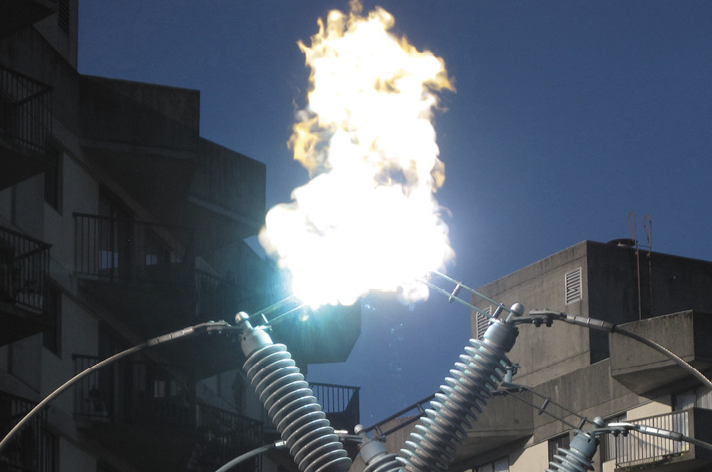
\includegraphics[width=0.87\linewidth]{images/Lichtbogen}
\caption[Lichtbogen]{Lichtbogen \autocite{Lichtbogen}}
\label{fig:Lichtbogen}
\end{figure}
\end{description}
Zudem sollen Sie die angeschlossenen Verbraucher in diesem Fall Häuser schützen. Eine ausgelöste Sicherung man schnell erkennen, da diese ein sogenanntes 
Fähnchen besitzt, welches sich bei Auslösung aufstellt. 
Dieser Mechanismus wird ausgelöst durch einen Draht, welcher mit dem Fähnchen verbunden ist und im inneren der Sicherung schmilzt, sobald der maximale Strom 
überschritten wird. Anschließend stellt sich dieses Fähnchen bzw. Metallplättchen durch einen federnden Mechanismus auf und signalisiert somit die Auslösung. 
Ein KVS ist wie im ersten Kapitel beschrieben eine Weiche, heißt eine Abzweigung von einem oder mehreren Kabeln auf ein Neues. In diesem KVS sind 
4 Kupferschienen installiert. Drei dieser Kupferschienen sind bestimmt für die drei Leiter im Dreiphasenwechselstrom und die übriggebliebene Schiene ist 
für den Schutzleiter (PEN). Diese Schienen nennt man auch Sammelschienen, weil dort die Leisten montiert sind. Jede Leiste hat die Funktion,
dass an diese die vier Adern des Kabels angeschlossen werden können und separat eingesichert werden können. Das Einsichern beschreibt den Prozess, in der 
man die Sicherungen in die Leisten hineinsteckt und somit eine Verbindung zwischen Kabel und Sammelschiene herstellt. Dieser Prozess ist enorm wichtig, da 
jede Leiste mit der Sammelschiene verbunden ist und durch das gezielte Einsichern verschiedene Kabel in Betrieb genommen werden können. Durch das Einsichern,
wird eine Verbindung zwischen der Sammelschiene und dem Kabel hergestellt. Diese Verbindung, welche über die Sicherung hergestellt wird, sorgt für eine 
Übertragung des Stroms. Jede Leiste hat ebenfalls einen Anschluss für den PEN-Leiter. Dieser ist zugleich der PE als auch der N Leiter in einem 
Dreiphasensystem und hat unter anderem die Aufgabe des Rückleiters bei einem unsymmetrischen Dreiphasenwechselstromverbrauch. Ein unsymmetrischer 
Verbraucher stellt \zB ein Haus dar, da jeder der drei Leiter mit einem unterschiedlichen Widerstand belastet wird und somit die Ströme der Leiter verschieden 
sind. Um nun einen möglichen Kurzschluss, heißt die Verbindung zwischen zwei stromführenden Leitern zu verhindern, müssen die KVS regelmäßig kontrolliert und 
gesäubert werden, sodass diese gar nicht erst entstehen kann. \autocite{Weigerber.2013}
\\\\ 
Eine weitere Maßnahme betrifft die Freileitungen im Stromnetz, da diese oftmals an Holzmasten befestigt sind und witterungsbedingt an Stabilität verlieren. 
Eine Freileitung ist definiert durch ein Kabel, welches an der freien Luft an einem Masten befestigt wird und entweder isoliert oder blank ist. Bei einem 
nicht isolierten, also blanken Kabel sind die einzelnen Adern aufgeteilt und in einem sicheren Abstand getrennt voneinander befestigt. Dies ist notwendig, 
um einen Kurzschluss zwischen den stromführenden Leitern, den Adern, zu verhindern. Um zu gewährleisten, dass die befestigte Freileitung Stürmen standhält,
müssen die Holzmasten kontrolliert werden. Dazu ist jeder Mast im System hinterlegt und muss nach einem festgelegten Protokoll geprüft werden. Darunter ist 
die Beschriftung, der Zustand, die Isolatoren und die Trassenart zu prüfen, sowie ob dieser einen Anker, eine Strebe, eine Kabelaufführung, einen 
Überspannungsableiter oder eine Erdung hat. Der Anker ist ein Stahlseil, welches an der Spitze des Masten befestigt wird und über einen Stahlstab im Boden 
befestigt ist. Er kompensiert die auftretenden Zugkräfte im Mast und verhindert so ein umkippen. Eine Zugkraft beschreibt die Kraft, welche auftritt, wenn 
an beiden Seiten eines Seils gezogen wird. 
\begin{figure}[hbt]
    \centering
    \includegraphics[width=1\linewidth]{images/Mastkräfte}
    \caption[Isolator]{Kräfte im Freileitungsmast (eigene Darstellung)}
    \label{fig:Kräfte im Mast}
\end{figure}
\\Auf dem Bild wird gezeigt, wie der Anker das Umkippen des Masts verhindert, indem er die entstehenden Zugkräfte durch die Freileitungsseile entlang des Ankers 
aufnimmt. Somit entsteht ein Kräftegleichgewicht zwischen der Seilkraft der Freileitung und der Zugkraft im Anker, womit der gemeinsame Punkt im Mast auf der 
Stelle gehalten wird und nicht wegkippt. Die Strebe ist ein zusätzlicher Holzmast, der schräg am eigentlichen Mast befestigt wird und dient ebenfalls zur 
Abstützung des Masts. Sie sorgt für die Aufnahme von Druckkräften, welche entstehen, wenn der Mast gegen die Strebe drückt. Diese Kräfte wollen die Holzstrebe
zusammendrücken und sorgen somit für den Namen der Druckkraft. Im Gegensatz zum Seil zieht der Mast nicht an der Strebe, sondern er drückt dagegen. Die 
Trasse beschreibt eine Freileitung, welche durch die Landschaft verläuft und kann unterschiedlich aussehen, deshalb ist es wichtig die Trassenart zu notieren,
um wichtige Informationen über die Anordnung der Seile zur Verfügung zu haben. Anschließend wird der Zustand des Masten geprüft, indem mit einem Hammer 
dagegen geklopft wird. So kann je nach Geräusch ermittelt werden, ob der jeweilige Mast morsch oder noch in Ordnung ist. Ein Mast kann morsch werden durch 
Verwitterung oder Tierbefall. Bei entsprechender Beschädigung muss der Mast ausgetauscht werden. Hierzu wird der Abschnitt, indem der Mast getauscht werden 
soll entsichert. Dies bedeutet, dass auf einem Stück zwischen zwei KVS die Sicherungen entfernt werden, sodass kein Strom mehr fließt und gefahrenfrei an 
der Freileitung gearbeitet werden kann. Anschließend ist es möglich den beschädigten Mast auszutauschen und den Abschnitt wieder in Betrieb zu nehmen. 
\begin{figure}[hbt]
    \centering
    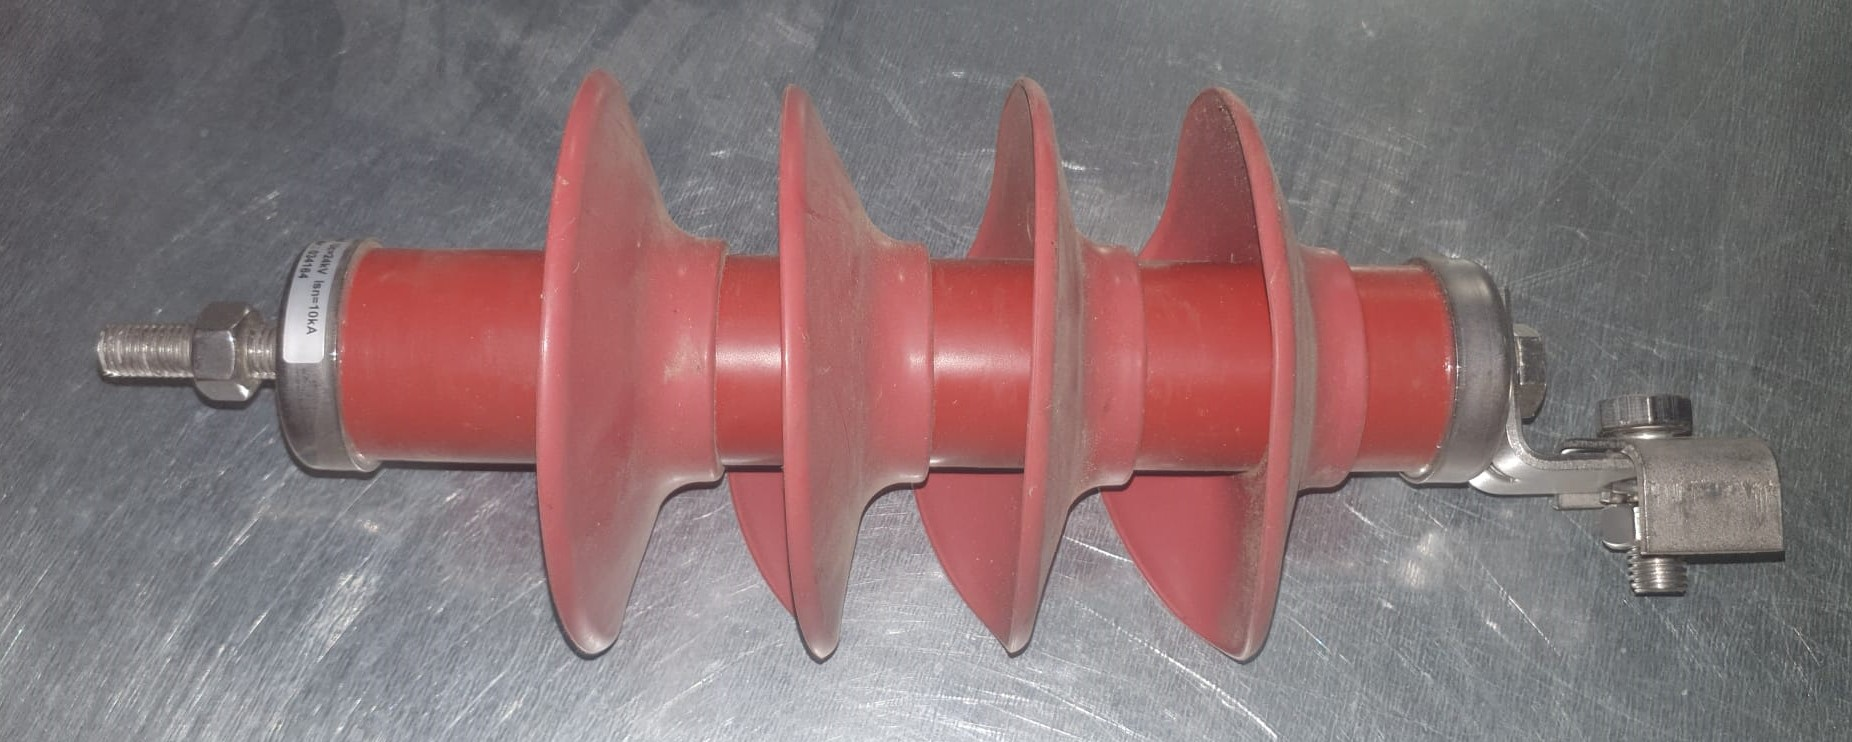
\includegraphics[width=0.98\linewidth]{images/Isolator}
    \caption[Isolator]{Freileitungsisolator (eigene Darstellung)}
    \label{fig:Isolator}
\end{figure}
\\Unter der Prüfung der Isolatoren versteht man die Sichtkontrolle auf Beschädigungen und die Notierung des Materials, da es entweder Keramik oder Kunststoff 
Isolatoren sein können. Diese haben den Nutzen, die unter Spannung stehenden Freileitungsseile vom Masten zu isolieren, sodass dieser nicht unter Spannung 
steht. Wie im Bild zu sehen, haben Isolatoren einen speziellen Aufbau, sodass der Strom den längst möglichen Weg überwinden muss, um an das andere Ende zu 
gelangen. Die tellerförmigen Ringe dienen zur Verlängerung des zurückzulegenden Wegs.Die Beschriftung eines Masten beinhaltet die Nummer, den Typ und die 
Höhe, welches wichtige Informationen zur Widererkennung darstellen. Eine Kabelaufführung beschreibt, wenn an einem solchen Mast ein Niederspannungskabel 
aus der Erde nach oben geführt wird und in eine Freileitung übergeht. Der Überspannungsableiter und die Erdung sind ein optionales Bauteil an einem Masten 
und sorgen bei Blitzeinschlag oder anderen Störungen in der Leitung für eine Ableitung der Spannung in die Erde.
\\
Im Mittelspannungsnetz werden häufiger Stahlmasten verwendet, welche ebenfalls einer solchen Kontrolle unterliegen. Dieses Netz besteht entweder aus Kabeln, 
welche im Erdreich verlegt werden oder aus den typischeren Freileitungen. Das Mittelspannungsnetz in Deutschland führt eine Spannung von 20.000 Volt (20 kV) 
und die Kabel haben nur die drei Adern L1, L2 und L3. Im Gegensatz zum Niederspannungsnetz, also bis 400 Volt, besitzen diese Leitungen keinen PEN Leiter, da 
es immer symmetrisch betrieben wird und kein direkter Verbraucher auf Ihnen hängt. Dies bedeutet, dass sich die Spannungen und Ströme gegenseitig aufheben, 
weil diese gleich groß und lediglich Phasenverschoben sind. Die Verschiebung der Phase kommt von der Erzeugung des Stromes, da sich im inneren eines Generators 
ein Magnet dreht, welcher zu unterschiedlichen Zeiten bei den drei Spulen vorbeikommt. Diese Spulen bestehen aus ringförmig aufgewickeltem Kupferdraht, welche 
auf das Magnetfeld des drehenden Magneten reagieren und die Elektronen in Bewegung bringen. Durch die Bewegung der Elektronen, also der kleinsten negativ 
geladenen Teilchen im Kupferdraht, entsteht eine Differenz in der Anzahl der Elektronen, welche sich im Draht befinden. Durch diese Differenz, auch 
Potentialdifferenz genannt, definiert sich eine messbare Spannung zwischen den zwei Enden des Drahtes. Diese Spannung wird nun im deutschen Stromnetz genutzt 
und über Kabel oder Freileitungen verteilt. Das eine allzeitige Versorgungssicherheit herrscht, müssen diese regelmäßig überprüft und im System aufgenommen 
werden, um eine schnelle Informationsbereitstellung bei Störungen zu gewährleisten. Hierzu wird jeder Mast im Freileitungsnetz auf Beschädigungen geprüft und 
es werden wichtige Informationen zur Höhe, Befestigungs-, Isolator- und Trassenart dokumentiert. Dies erfolgt nach dem oben genannten Mastprotokoll und wird 
in regelmäßigen Abständen durchgeführt. Außerdem ist wichtiger Bestandteil dieser Kontrolle, dass überprüft wird, ob Äste in die blanken Seile hineinhängen, 
da diese bei Berührung oder Annäherung zu einem Kurzschluss oder Brand führen können. Um dies zu vermeiden, werden bekannte Stellen frühzeitig von Ästen 
befreit und neu gemeldete Orte kontrolliert und ggf. freigeschnitten. Dieses Freischneiden mit Hilfe von Forstwerkzeugen, wie Kettensägen oder Handsägen, 
wird ausasten genannt.
\\
Nicht nur Freileitungen oder KVS müssen kontrolliert werden, sondern auch die Schnittstellen zwischen Nieder- und Mittelspannungsnetz. Diese Umspannstationen 
transferieren die Mittelspannung mit Hilfe von Transformatoren zu Niederspannung. Ein Transformator ist ein Bauteil im Stromnetz, welches dafür sorgt eine 
Eingangsspannung \zB 20 kV umzuwandeln in eine Ausgangsspannung von 0,4 kV. Dazu besitzt dieser einen Eisenkern, der mit zwei verschiedenen Spulen 
umwickelt ist, an diese dann die Mittel- und Niederspannung angeschlossen werden kann. Durch die unterschiedliche Wicklungszahl der beiden Spulen ist 
es möglich die Spannung zu verringern. Mit folgender Formel kann berechnet werden, wie hoch die Wicklungszahl sein muss, wenn man \zB eine 
Eingangsspannung $U_1$ auf eine Ausgangsspannung $U_2$ transferieren möchte. 
\begin{equation}
\frac{U_1}{U_2}=\frac{w_1}{w_2}
\label{eqn:Transformator Wicklungszahl}
\end{equation}
Stellt man eine Rechnung zu einem alltäglichen Gebrauch der TWS Netz GmbH auf, in dem eine 20 kV Einspeisung in eine 0.4 kV Spannung umgewandelt werden 
soll, dann kommt man auf folgende Rechnung:
\begin{eqnarray}
\frac{w_1}{w_2}=\frac{U_1}{U_2}=\frac{20000\text{V}}{400\text{V}}=50
\label{eqn:Beispiel Wicklungen}
\end{eqnarray}
\\
Diese sagt nun aus, dass ein Transformator ein 50-faches Verhältnis der Spulenwicklungen benötigt, um Mittelspannung in Niederspannung zu transferieren. Diese 
unterschiedlichen Spannungen müssen getrennt voneinander sein und dürfen lediglich über die Spulen magnetisch gekoppelt werden. Dazu muss es in den 
Umspannstationen trocken und sauber sein, da sonst die Gefahr herrscht, dass eine leitende Verbindung zwischen Mittel- und Niederspannung hergestellt wird. 
Dies hätte zur Folge, dass es zu einem Kurzschluss kommt und der Transformator zerstört wird. Um es gar nicht erst soweit kommen zu lassen, müssen Umspannstationen 
bei Besuch sauber gehalten werden und bei festgestelltem Feuchtigkeitseintritt so schnell wie möglich renoviert werden. \autocite{Weigerber.2013} 
\\
Zudem gibt es auch im Mittelspannungsnetz Abzweige zwischen verschiedenen Kabeln. Diese Abzweige werden in Schaltwerken realisiert. Sie funktionieren wie ein 
großer Bahnhof, in dem einzelne Mittelspannungskabel, von \zB Umspannwerken oder anderen Mittelspannungskreisen hineinkommen und auf einer Sammelschiene, 
ähnlich wie im KVS zusammenlaufen. Von dieser Sammelschiene aus können Kabel abgehen und neue Stromkreise bilden. Diese sind deutlich aufwendiger zu schalten, 
da es in diesem Netz keine Sicherungen zum umschalten verschiedener Kabel gibt, sondern nur die sogenannten Lasttrennschalter. Diese funktionieren wie 
Lichtschalter, in denen  eine Metallstange zwischen die beiden Kontakte geschaltet wird, sobald man diesen einschalten möchte. Hierbei wird zwischen zwei 
Typen unterschieden, dem luft- und dem gasisolierten Trennschalter. 
Der luftisoliere Lasttrennschalter ist sehr pflegeleicht, da man ihn nur selten prüfen 
muss und dieser langlebig in seiner Funktion ist. Er muss lediglich ausgetauscht werden, wenn ein defekt im Schaltvorgang vorliegt, \zB der Metallschalter 
schließt nicht mehr mit den Kontakten. Bei den gasisolierten Schaltanlagen muss darauf geachtet werden, dass der Gasdruck immer ausreichend hoch ist, da 
diese auf wesentlich kleinerem Raum gebaut sind und somit nur durch das Gas isoliert werden. Diese Schalter funktionieren gleich, wie die luftisolierten, 
allerdings wird das Gas Schwefelhexafluorid (\ce{SF_6}) angewandt um eine Isolierung zu schaffen. Dies hängt mit der engen Bauweise der Anlagen zusammen und hätte 
ohne Gasisolierung die Folge, dass der Strom von dem einen auf den anderen Schalter überschlägt und einen Kurzschluss erzeugt. Ein Überschlag ist eine 
Verbindung zwischen zwei Leitern über die Luft mit Entstehung eines Lichtbogens und ohne direkten Kontakt der Leiter. Fällt bei Kontrolle dieser \ce{SF_6} Zelle 
auf, dass der Druck zu gering ist, muss diese ausgetauscht werden durch eine neue Zelle.
Eine Zelle definiert sich durch einen Block, indem sich drei Schalter 
für ein Mittelspannungskabel mit drei Adern befinden. \ce{SF_6} ist ein chemisch hergestelltes Gas, welches sehr gut isoliert und daher oft bei Schaltern für 
Mittel- und Hochspannungsanagen eingesetzt wird. Dieses Gas hat den großen Nachteil, dass es schlecht für die Umwelt ist, weil es zur Erderwärmung beiträgt, 
wenn es freigesetzt wird. Daher sind die \ce{SF_6} Schalter luftdicht abgekapselt zur Zelle selbst, um jeglichen austritt des Gases zu verhindern. Beim Austausch 
muss die alte Zelle zum Hersteller oder zu zertifizierten Recyclingunternehmen zurückgebracht werden, um das noch vorhandene Gas rückzugewinnen und die 
Umwelt zu schützen. \autocite{Schwab.2012}
\clearpage

\section{Maßnahmen zur Erhaltung der Versorgungssicherheit}

Die Kontrolle und Pflege des Nieder- und Mittelspannungsnetzes der TWS Netz GmbH hat eine große Bedeutung für die Versorgungssicherheit im gesamten 
Versorgungsgebiet. Wie vorherig erläutert, benötigt es eine strukturierte und regelmäßige Begehung der kritischen Punkte im Netz. Dazu zählen vor allem die 
Freileitungsmasten aus Holz, wie auch die Ust., da Sie die Knotenpunkte im gesamten Netz darstellen. Durch die Versorgung der Ust. mit Mittelspannung, ist es 
überhaupt möglich ein Niederspannungsnetz zu betreiben. Um dies zu vermeiden werden regelmäßige Inspektionen, Wartungen und Überprüfungen durchgeführt. 
Zudem ist es wichtig, dass Stromnetz fortschreitend zu erneuern, um Schwachstellen früh genug zu erkennen und zu beseitigen. Aber nicht nur die Betreuung 
der Mittelspannung ist von Relevanz, sondern auch die Pflege des Niederspannungsnetzes, da hier die Verbraucher direkt angeschlossen sind und am schnellsten 
von Ausfällen betroffen sind. Dies wird durch die gezielte Pflege, Kontrolle und Instandhaltung erreicht, um den Kunden immer eine funktionierende 
Stromversorgung zu gewährleisten. Diese ist wichtig, um ein positives Image und eine zukunftsfähige Wirtschaftlichkeit zu erreichen. Andernfalls kommt es zu 
einem Kundenrückgang, welcher die Zukunft des Unternehmens gefährdet. Des Weiteren sind Kontrollen bei \ce{SF_6} Anlagen enorm wichtig, da es sich um 
umweltschädliche Substanzen handelt und diese Auflagenkonform betrieben werden müssen, um die daraus folgenden Umweltbelastungen zu minimieren. Grundlegend 
wurden Strukturen zu verschiedenen Betriebsaufgaben, welche zielführend für ein stabiles Stromnetz sind, erlernt. Dazu wurden die Vorgehensweisen unter 
realen Bedingungen angewandt und vertieft.
\clearpage
%%%%%%%%%%%%%%%% Nächste Tätigkeit %%%%%%%%%%%%%%%%

\section{Installation verschiedenster Kabelmuffentypen}

Zu den Haupttätigkeitsbereichen des Betrieb Stromnetzes gehören die Kabelverbindungen, Kabelabzweige und Kabelenden, auch Muffen genannt. Diese bringen die 
Aufgaben der Installation mit sich und können je nach Anwendungsbereich verschiedene Arten der Installation aufweisen. Dazu zählen \zB die Verbindungsmuffen, 
die Abzweigmuffen, aber auch spezielle Übergangsmuffen oder Kabelenden im Bereich der Nieder- und Mittelspannung. Zudem unterscheiden sich die 
Kabelverbindungen im Niederspannungsnetz, mit denen im Mittelspannungsnetz, da dort viel höhere Anforderungen an die Verbindungen gestellt werden und eine 
höhere Sicherheit vonnöten ist. Um solch eine Qualität zu gewährleisten muss vorausgesetzt werden, dass jeder Mitarbeiter über die Vorgehensweise und den 
Umgang mit Material, sowie mit Gefahrstoffen informiert ist und dies bei seinem Problem anwenden kann. Diese Problemstellungen können sich unterscheiden von 
einem einfachen verbinden zweier Kabel, über den Übergang von verschiedenen Kabelquerschnitten, wie auch ein Abzweig von einem auf zwei neue Kabel. Bei 
Mittelspannungskabeln fällt der Abzweig weg, da dies technisch nicht möglich ist und somit in einem Schaltwerk oder in einer Ust. durch Lasttrennschalter 
erfolgt. Zudem fallen auch Kabelenden in den Bereich der Kabelmuffen. Hierbei wird zusätzlich unterschieden zwischen spannungsfesten und spannungsfreien 
Kabelenden. 
\\
Ziel ist das Installieren von Kabelmuffen verschiedenen Typs. Zudem soll erlernt werden, wie diese bei verschiedenen Kabeln anzuwenden sind und was dabei 
zu beachten ist.
\clearpage

\section{Stromnetzerweiterungen und -erneuerungen durch die Kabelmuffentechnik}

Die erste Art der Kabelmuffen, ist die Verbindungsmuffe. Diese dient zur unterbrechungsfreien Verbindung zweier Kabel und findet meist ihren Einsatzbereich 
in der Verlängerung oder Reparatur vorhandener Kabel. Zudem kann diese Art der Muffe flexibel eingesetzt werden und bietet zwei verschiedene Methoden zur 
Montage. Eine dieser Methoden ist die Warmschrumpftechnik, in der die zusammengefügte Stelle mit Hilfe von Schrumpfschläuchen isoliert wird. Der Begriff 
warmschrumpfen kommt vom Schrumpfen der Schläuche durch Hitze. Dieses sogenannte Schrumpfen beschreibt den Prozess, in dem sich der Kunststoffschlauch 
aufgrund seiner chemischen Eigenschaften als Thermoplaste zusammenzieht und nach abkühlen seine Form beibehält. Diese Eigenschaft der Umformbarkeit bei 
Wärmezufuhr beschreibt die thermoplastischen Kunststoffe. Um nun die beiden Kabel zu verbinden, werden sogenannte Schraubverbinder eingesetzt. Diese können 
auf ein abisoliertes Kabelende geschraubt werden und stellen eine Verbindung zwischen den Kabeln her. $\text{mm}^2$
\begin{figure}[hbt]
\centering
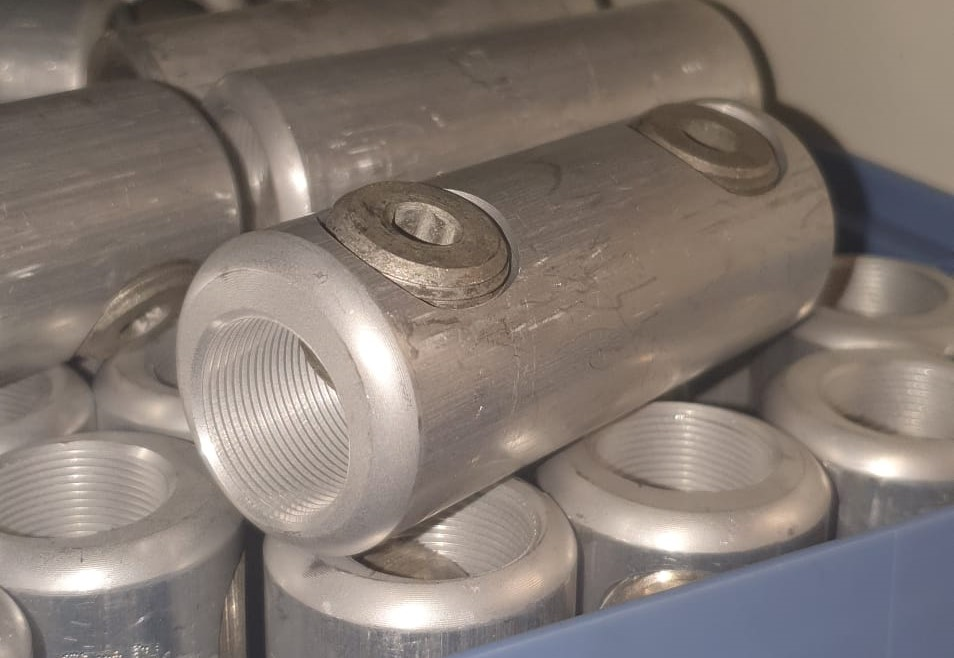
\includegraphics[width=0.98\linewidth]{images/Schraubverbinder}
\caption[Schraubverbinder]{Schraubverbinder Niederspannung}
\label{fig:Schraubverbinder}
\end{figure}
\\
Der auf dem Bild zu sehende Schraubverbinder, wird ausschließlich im Bereich der Niederspannung eingesetzt, da dieser bis zu einem maximalen Aderquerschnitt 
von 150 $\text{mm}^2$ und 1 kV maximale Spannung einsetzbar ist. Dies ist ausreichend, da im Niederspannungsnetz der TWS Netz GmbH ein Aderquerschnitt von 
max. 150 $\text{mm}^2$ eingesetzt wird. Dieser Aderquerschnitt, auch als Nennquerschnitt eines Kabels bezeichnet, gibt die dicke einer einzelnen Ader an, mit Hilfe 
der sichtbaren Fläche beim durchtrennen einer Ader. Meist kommt vor diese Angabe noch eine andere Zahl, welche angibt, wie viele Adern ein Kabel hat. Eine 
solche Bezeichnung sieht wie im folgenden Beispiel aus: 4x150 $\text{mm}^2$. Zur Installation werden die Schraubverbinder auf alle vier Adern eines Erdkabels des 
Typs NAYY geschraubt und anschließend mit separaten Schrumpfschläuchen isoliert, um einen Kurzschluss zwischen den Leitern zu verhindern. Dieser Erdkabeltyp 
besteht aus vier Aluminiumleitern, welche einzeln isoliert sind und durch eine zusätzliche Füllung zwischen Außenmantel und Aderisolierung vor Verdrehung 
geschützt werden. \autocite{NKT_NAYY}
\\
Um den Außenmantel zu ersetzen, wird bei einer Verbindungsmuffe ein großer Schrumpfschlauch über beide Kabel abgeschrumpft, um das gesamte Muffenpaket zu 
schützen, wenn es in der Erde liegt. Das Muffenpaket definiert sich aus dem Bündel der vier Schraubverbinder einer Verbindungsmuffe, den abgemantelten Adern 
der Kabel und dem darüber abgeschrumpften Mantelschlauch. \autocite{Cellpack}
\\
Die Verwendung von Aluminiumkabel sind im Stromnetz geläufiger, als die Verwendung von Kupferkabeln, da diese ein leichteres Gewicht aufweißen und Aluminium 
kosteneffizienter ist. Vergleicht man dieses Gewicht eines Aluminiumkabels des Typs NAYY mit einem Kupferkabel des Typs NYY, dann kommt man auf eine 
Reduzierung des Gewichts durch den Aluminiumleiter von ca. 3,5 Tonnen pro Kilometer Kabel. Der preisliche Unterschied des Kupferkabels in Verbindung mit dem 
geringfügigen kleineren Leitungswiderstand ist nicht wirtschaftlich genug, um dem im Vergleich stehende Aluminiumkabel stand zu halten. \autocite{NKT_NYY}
\\
Dieser Leitungswiderstand kann berechnet werden, mit Hilfe des spezifischen Widerstandes, dem Querschnitt und der Länge des Kabels. 
\clearpage
Der spezifische Widerstand ist eine konstante Größe für unterschiedliche Materialien und kann in folgender Tabelle abgelesen werden.
\begin{table}[hbt]	
	\centering
	\renewcommand{\arraystretch}{1.5}
	\captionabove[Materialkonstanten]{Materialkonstanten \autocite{Weigerber.2018}}
	\label{tab:Materialkonstanten }
	\begin{tabular}{|c|c|c|c|c|}
        \hline
		\textbf{Material} & \textbf{Symbol} & \textbf{spez. Widerstand} & \textbf{spez. Leitwert} & \textbf{Temperaturkoeffizient}\\
        \textbf{} & \textbf{} & \textbf{in} $\mathbf{\frac{\Omega \cdot \textbf{mm}^2}{\textbf{m}}}$ & \textbf{in} $\mathbf{\frac{\textbf{m}}{\Omega \cdot \textbf{mm}^2}}$ & \textbf{in} $\mathbf{\frac{1}{^\circ \textbf{C}}}$ \textbf{oder} $\mathbf{\frac{1}{\textbf{K}}}$\\
		\hline 
		Aluminium   & \ce{Al}               &   0,028 &   36    & 0,004     \\
		\hline 
        Silber      & \ce{Ag}               &   0,016 &   63    & 0,004     \\
        \hline
        Kupfer      & \ce{Cu}               &   0,018 &   56    & 0,004     \\
        \hline
        Gold        & \ce{Au}               &   0,023 &   44    & 0,004     \\
        \hline
        Platin      & \ce{Pt}               &   0,11  &   9     & 0,002     \\
        \hline
        Eisen       & \ce{Fe}               &   0,125 &   8     & 0,005     \\
        \hline
        Manganin    & \ce{Cu, Fe, Mn, Ni}   &   0,4   &   2,5   & 0,00001   \\
        \hline
        Chromnickel & \ce{Cr, Ni, Fe}       &   1     &   1     & 0,00005   \\
        \hline
	\end{tabular} 
\end{table}
Anschließend kann mit Hilfe der folgenden Formel ein Leitungswiderstand für unterschiedliche Materialien, Querschnitte und Längen berechnet werden.
\begin{equation}
R_a=\frac{\rho \cdot l}{A}=\frac{l}{\kappa \cdot A}
\label{eqn:Leitungswiderstand}
\end{equation}
Dieser Muffentyp wird auch im Bereich der Mittelspannung verwendet, da es die beste Variante zur Verbindung zweier Kabel darstellt. Hier ist die Installation 
allerdings deutlich komplizierter, da die Verbindung höheren Spannungen standhalten und zudem auch noch besser isoliert werden muss, um Kurz- und Erdschlüsse 
zu vermeiden. Ein Erdschluss ist eine elektrische Verbindung zwischen stromführendem Leiter und der umliegenden Erde. Je nach Kabel Typ unterscheidet sich der 
Aufwand, um die Verbindungsmuffe zu installieren. Meist wird diese jedoch bei Kunststoffkabeln angewandt, welche drei einzelne Leiter eines bestimmten 
Querschnitts aufweisen. Ein solches Kabelbündel hat die Bezeichnung 3x1x300 mm$^2$ und sagt aus, dass es drei einzeln isolierte Leiter des Nennquerschnitts 
300 mm$^2$ sind. %Bild_MS_Kabel% 
Jedes einzelne Kabel benötigt somit eine eigene Muffe, welche nach Einhaltung der Anleitung installiert werden muss. Dies ist von enormer Wichtigkeit, da jede 
Produktionsreihe andere Vorgehensweisen zur Installation aufweisen kann und somit Fehler und Sicherheitsrelevante Probleme entstehen können. Dies betrifft 
vor allem die exakte Länge der abzumantelnden Bereiche und Schichten der Isolierung, da Mittelspannungskabel verschiedene Isolierungsschichten besitzen, um 
den Leiter zu schützen. Ein Kabel des Typs NA2XS(F)2Y hat \zB sieben Schichten um den Leiter herum. Dazu zählen drei leitfähige Schichten, welche dafür 
sorgen, dass die Spannung an die Isolierung geleitet wird und zwei Kunststoffisolierungsschichten. Die innere der beiden stellt eine Isolierung zwischen dem 
Leiter und Kupferdrahtschirm her und die äußere stellt den Mantel dar, welcher das Kabel hauptsächlich vor äußeren Einflüssen schützt. Der sogenannte 
Kupferdrahtschirm ist bei Mittespannungskabeln eine zusätzliche Erde und dient zudem auch noch zur Abschirmung von elektrischen Feldern. \autocite{NKT_NA2XSF2Y}
Diese elektrischen Felder 
entstehen bei jedem stromdurchflossenen Leiter und müssen vor allem bei Mittelspannung eingedämmt werden. Um bei einer Verbindung zweier Leiter 
sicherzustellen, dass die Verbindung des Kupferdrahtschirmes besteht, muss dieser ebenfalls verbunden werden. Dies erfolgt meist durch einen kleinen 
Schraubverbinder. Der Aluminiumleiter selbst, wird durch einen großen Schraubverbinder, mit Hilfe von vier Schrauben verbunden. Diese Schrauben brechen an 
einem bestimmten Punkt von selbst ab, um immer ein ähnliches Drehmoment zu erreichen. Ein Drehmoment beschreibt die aufzuwendende Kraft bei einer Drehung 
einer Schraube. Nach installieren des Schraubverbinders, ist es wichtig jeglichen Freiraum mit beiliegendem Füllmaterial zu füllen, um jegliche 
Lufteinschlüsse zu vermeiden. Diese Lufteinschlüsse in einer Mittelspannungsverbindung würden zu Geräuschen im Isolator des nächstliegenden Schaltwerks führen 
und sind zu vermeiden. Anschließend wird ein Schrumpfschlauch, welcher für 20 kV geeignet ist über der Verbindung abgeschrumpft, um diese vor Kurzschlüssen zu 
schützen. Zuletzt ist es noch wichtig einen Mantelschrumpfschlauch über dem Paket aus Schraubverbinder und Kupferschirm abzuschrumpfen, um die gesamte Muffe 
vor äußeren Einflüssen zu schützen. Da Mittelspannungskabel drei dieser Kabel für die Phasen L1, L2 und L3 besitzen, muss dieser Prozess dreimal wiederholt 
werden um eine Verbindung herzustellen. Eine weitere Methode stellt die Gießharzmethode dar, in der als Isolator ein Harz verwendet wird, welches in eine Form 
gegossen und anschließend ausgehärtet wird. Dieses Harz besteht aus einer zwei teiligen chemischen Mischung, welche nach vermischen miteinander reagiert und 
zu einer aushärtenden Kunststoffmasse wird. Diese Masse ist letztendlich isolierend und schützt nach Aushärtung die Muffe vor äußeren Einflüssen. Diese Methode 
wird nur noch bei Abzweigmuffen verwendet, da dass Schrumpfverfahren deutlich schneller und einfacher anzuwenden ist. \autocite{Cellpack}
\\\\
Im Stromnetzerneuerungsprogramm der TWS Netz GmbH werden lang bestehende Kabelstrecken ersetzt. Dabei müssen Kabel mit verschiedenen Eigenschaften und 
Querschnitten verbunden werden. 
Die Kabelauftrennung findet ihre Anwendung bei Kabeln des Typs N(A)KBA, welche alle drei Adern in einem Kabel besitzen und für den Übergang auf einen aktuell 
verwendeten Kabeltypen, welcher im dreier Bündel vorhanden ist, erst aufgetrennt werden muss. Da ein Kabel des Typs N(A)KBA mit ölgetränktem Papier, einem 
Bleischirm und einem Jutemantel, heißt einem aus Pflanzen hergestelltem Stoff, isoliert ist, muss vor allem auf umweltgerechte Entsorgung und fachgerechtes 
Arbeiten unter der Benutzung von PSA geachtet werden. Zudem wird nach entfernen der Isolierung und auftrennen der einzelnen Adern eine abschrumpfbare 
Ölstoppkappe installiert, um austretendes Öl zu verhindern und weitere Schädigung der Umwelt einzudämmen. Da dieser Kabeltyp meist einen im Verhältnis sehr 
kleinen Nennquerschnitt hat, muss zudem eine Übergangsmuffe zum erhöhen des Kabelquerschnitts installiert werden. Diese Art der Muffe wird äquivalent zu 
einer Verbindungsmuffe installiert. Allerdings hat diese den entscheidenden Unterschied, dass der Schraubverbinder einschraubbare Plastikeinsätze hat, um auch 
kleinere Kabelquerschnitte zentriert einzuführen und festzuschrauben. Durch die Zentrierung ist gewährleistet, dass das Kabel immer mittig im Schraubverbinder 
liegt und nicht bei der Installation verrutscht. Diese Übergangsmuffen gibt es für verschiedene Kabeltypen und sind je nach Problemstellung auch mehrfach, \zB 
um einen Zwischenübergang von 95 mm$^2$ auf 185 mm$^2$ zu schaffen, um dann auf 300 mm$^2$ zu verbinden. Kabelverbindungsmuffen und Übergangsmuffen tragen im 
Mittelspannungsnetz einen wichtigen Anteil in der Versorgungssicherheit, da Sie für die Versorgung von Ust. verantwortlich sind und zur Erneuerung und 
Instandhaltung des Bestandsnetzes beitragen. \autocite{Cellpack}
\\
Ein weiterer Muffentyp ist die Abzweigmuffe, welche ausschließlich im Niederspannungsnetz verwendet wird und nur in der Gießharzmethode verbaut wird. Diese 
Muffenart dient dazu eine Abzweigung des Stromkabels zu schaffen um beispielsweise einen Haushalt anzuschließen. Für die Montage einer Abzweigmuffe wird beim 
Bestandskabel lediglich der Mantel, heißt die äußere Isolierschicht entfernt, um die einzelnen Adern freizulegen. Um nun einen Abzweig zu schaffen, wird mit 
Hilfe einer Kabelabzweigklemme ein Kontakt zum Bestandskabel hergestellt. Diese Abzweigklemme hat spitzen, welche sich bei der Montage, also dem festschrauben 
der Klemme um die Adern, durch die Isolierung drücken und sich in den Aluminiumleiter hineintreiben. Durch diese Kontaktpunkte kann nun der Strom fließen und 
somit können auch die einzelnen Adern in der richtigen Zuordnung an diese Klemme angeschlossen werden. Zuletzt muss noch die entfernte Isolierung 
wiederhergestellt werden. Dies erfolgt durch eine Plastikform, welche um das Abzweigbündel montiert und abgedichtet wird, sodass in diese das Gießharz 
eingefüllt werden kann. Nach Aushärtung stellt dieser Schutz aus Gießharz die neue Isolierung dar und sorgt für einen Schutz der betroffenen Stelle. Diese 
Art der Muffe hat eine wichtige Bedeutung im Stromnetz, da man es mit Ihr flexibel erweitern kann und somit wenig Aufwand betreiben muss, um \zB neue Häuser 
an das Netz anzuschließen. \autocite{Cellpack}
\\\\
Ein letzter Typ der auch zu den Kabelmuffen zählt, ist das Kabelende. Dieses gibt es in zwei verschiedenen Ausführungen, dem spannungsfesten und 
spannungsfreien Kabelende. Das spannungsfeste Kabelende wird verwendet, um unter Spannung stehende Kabelenden zu isolieren gegen Kurzschluss und zusätzlich 
zu schützen vor Korrosion oder Beschädigung im Erdreich. Ein Kabel, bzw. der metallische Leiter kann durch eintretende Feuchtigkeit oder dem 
Umgebungssauerstoff in der Erde korrodieren, heißt sich zersetzen oder verrosten. Dadurch kann dieser unbrauchbar werden und muss somit durch ein Kabelende 
geschützt werden. Ein Kabelende kann gezielt verlegt werden, wenn \zB bekannt ist, dass in geraumer Zeit das Netzgebiet an dieser Stelle erweitert wird oder 
es kann entstehen durch die Erneuerung alter Kabel. Hierbei wird das alte Kabel meist nicht komplett aus dem Erdreich entfernt und wird nur versiegelt durch 
ein Kabelende. So ist gewährleistet, dass das Erdreich durch evtl. austretende Öle geschützt ist und das Kabel nicht korrodiert. Steht das Kabel unter 
Spannung muss darauf geachtet werden, dass ein spannungsfestes Kabelende montiert wird. Dieses unterscheidet sich zum normalen Kabelende darin, dass jede 
Ader einzeln mit einer schrumpfbaren Plastiktülle versiegelt wird und somit ein Kurzschluss zwischen den Adern vermieden wird. Eine Plastiktülle ist ein 
Plastikschlauch, der an einem Ende verschlossen ist und wie eine Kappe über der Ader montiert wird. Um zusätzlich das austretende Öl von alten Kabeln zu 
stoppen und die offenen Adern bei \zB spannungsfesten Kabelenden zu schützen, wird eine Endkappe über dem gesamten Kabel abgeschrumpft. Diese Endkappe ist 
bei spannungsfreien Kabelenden ausreichend und benötigt keine zusätzlichen Adertüllen. \autocite{Cellpack}
\\\\
Allerdings bringen diese Muffen auch Nachteile mit sich, denn sie stellen immer eine Schwachstelle im Netz dar. Kleinste Fehler in der Montage können dazu 
führen, dass die Isolierung nicht komplett wasserdicht ist und somit über die Zeit Wasser eintritt und die Muffe langsam kaputt geht. Dieses Wasser sorgt 
für kleinere Kurzschlüsse zwischen den Phasen, in denen zusätzlich Lichtbögen entstehen und den Leiter langsam schmelzen, bis dieser keinen Kontakt mehr hat. 
Deshalb muss die Anzahl der Muffen so gering wie möglich gehalten werden, um die Schwachstellen zu minimieren und somit eine Versorgungssicherheit 
herzustellen. 
\clearpage

\section{Die Bedeutung von Kabelmuffen im Stromnetz}

Das Muffen von Kabeln im Nieder- und Mittelspannungsnetz stellt für Netzerweiterungen und -erneuerungen im Stromnetz der TWS Netz GmbH eine grundlegende 
Tätigkeit zur Erhaltung der Stromversorgung dar. Bei falscher Montage können diese zu Störquellen im Stromnetz führen und müssen ausgetauscht werden. Dies 
hat zur Konsequenz, dass die betroffenen Stromkunden für einen gewissen Zeitraum keinen Strom haben, was negative Auswirkungen auf das Image mit sich ziehen 
kann. Zudem möchte man den Kabelwiderstand so gering wie möglich halten, um Leistungsverluste durch Kabelwiderstände zu minimieren. Aber auch für den 
Umweltschutz sind \zB Übergangsmuffen sehr wichtig, da andernfalls Öl aus alten Kabeln in das Erdreich sickern und dieses belasten würde. Zudem sind diese 
auch wichtig, wenn verschiedene Kabelquerschnitte verbunden werden, da nur sie für einen reibungslosen Übergang sorgen. Je nach Problemstellung gibt es 
verschiedene Techniken zur Installation, zwischen denen man auswählen kann. Dazu zählen die Warmschrumpf- oder Gießharztechnik. Beide Techniken wurden 
individuell an praktischen Problemen, wie \zB Verbindungs-, Übergangs- und Abzweigmuffen angewandt. Zudem wurden die wichtigsten zu beachtenden Regeln 
erlernt, um jegliche Art der Kabelmuffe anwenden zu können.
\clearpage
%%%%%%%%%%%%%%%% Nächste Tätigkeit %%%%%%%%%%%%%%%%

\section{Inspektion von Schaltfeldern im Stromnetz der TWS Netz GmbH}

Ein wichtiger Tätigkeitsbereich in der TWS Netz GmbH betrifft die Schaltfelder. Diese haben die Aufgabe, dass sie kleinere Gebiete im Stromnetz versorgen. 
Dabei hat jedes Schaltfeld einen eigenen Transformator, der für die Stromversorgung sorgt. Eine der Hauptaufgaben ist es, diese Schaltfelder zu inspizieren, 
um zu gewährleisten, dass jedes intakt ist und mit dem richtigen Transformator verschalten ist. Sollte dies nicht der Fall sein, muss dass Schaltfeld geändert 
werden. Änderungen können aber auch baubedingt vorgenommen werden und müssen ebenfalls überwacht und nach den Baumaßnahmen zurückgeschalten werden. Es kann 
allerdings auch eine neue Verschaltung vorgenommen werden, wenn es von Nöten ist. Diese Aufgabe der richtigen Aufteilung von einem in zwei Schaltfelder 
gehört auch zum Aufgabenbereich des Stromnetzmonteurs und wird oftmals in der Niederspannung durchgeführt. Zu diesen Aufgaben gehören \zB die Auftrennung, 
die Dokumentierung und die Erneuerung der Informationsmedien. Schaltfeldänderungen im Mittelspannungsnetz werden nur durchgeführt, wenn ein Stück der 
Leitung durch Baumaßnahmen ausgeschalten werden muss. Die Aufgabe besteht dann darin die Schaltung durchzuführen und ggf. noch ein Mittelspannungskabel zu 
schneiden. Grundlegend soll erlernt werden, wie sich die Schaltfelder untereinander Verhalten und welche Dinge wichtig zu beachten sind, um bei jeder 
Aufgabenstellung eine möglichst geringe Netzbeeinträchtigung zu haben. 
\clearpage

\section{Effiziente Schaltfeldverwaltung}

Das Niederspannungsnetz der TWS Netz GmbH unterteilt sich in eine Vielzahl von Schaltfeldern. Jedes Schaltfeld hat die Aufgabe einen kleinen Bereich im Gebiet 
abzudecken. Dabei teilt sich das Stromnetz in viele verschiedene Zweige, mit Hilfe von KVS und Umspannstationen auf. Da jeder KVS nur eine begrenzte Anzahl an 
Leisten hat, wie in Kapitel 2 erläutert und jeder Trafo nur eine begrenzte Leistung liefert, muss das Stromnetz unterteilt werden. Diese Unterteilung wird 
realisiert durch Schaltfelder, welche voneinander getrennt sind. Die Trennung der Schaltfelder untereinander spielt eine wichtige Rolle, da es im Falle einer 
Störung nur ein bestimmtes Schaltfeld betrifft. Somit kann die Störquelle eingegrenzt werden und es sind nur wenige Haushalte betroffen. Diese Auftrennung 
wird meist in KVS vorgenommen, da diese an andere Schaltfelder angrenzen. In diesen KVS finden sich nicht nur die Kabel des zugehörigen Schaltfeldes, sondern 
meist auch noch ein Kabel des angrenzenden Schaltfeldes. Dies hat den Hintergrund, dass bei einem Störungsfall oder Bauarbeiten die Leistung des Schaltfeldes 
erhöht oder gar ersetzt werden kann, wenn \zB arbeiten am Trafo stattfinden und dieser sein Schaltfeld nicht versorgen kann. Jeder Trafo hat eine vorgegebene
Nennleistung, mit der er bemessen wird. Diese Nennleistung bringt zur Aussage, wie viel Leistung ein Trafo übertragen kann, ohne etwas zu verbrauchen. Diese 
Leistung wird als Scheinleistung bezeichnet und hat die Einheit kVA. Diese beinhaltet die Wirkleistung und die Blindleistung. Die Wirkleistung bezieht sich 
auf die Leistung, die ein Verbraucher im Betrieb benötigt und wird in Watt (W) angegeben. Diese Leistung bezieht sich auf einen reellen Verbrauch, heißt auf 
einen rein ohmschen Widerstand. Die Blindleistung hingegen ist die verbrauchte Leistung durch Verschiebung der Phase und wird in var angegeben. \autocite{Hufschmid.2021} 
\\
Diese entsteht an der Ausgangsseite des Trafos durch unsymmetrische Verbraucher und kann variieren. Um einen Trafo richtig zu bemessen in der Leistung wird 
dieser in VA angegeben, um die Verluste durch Blindleistung mit einzubeziehen. Je nach Größe des Trafos hat dieser unterschiedlich hohe Bemessungen, welche 
in der Dimensionierung des Schaltfeldes beachtet werden müssen. Die Dimensionierung beschreibt die Festlegung bestimmter Größen eines technischen Produkts, 
um die geforderten Probleme zu erfüllen. Diese entscheidet letztendlich darüber, wie viele Verbraucher über das Stromnetz an den Trafo angeschlossen werden 
können, ohne diesen zu überlasten. Ein Trafo kann grundsätzlich in einer Notsituation überlastet werden, allerdings funktioniert dies nur über einen kurzen 
Zeitraum und in einem gewissen Maß. Eine zu lange Überlastung würde zu einer Überschreitung der Grenztemperatur führen und hätte zur Folge, dass die 
Isolierfähigkeit des isolierenden Öls im inneren des Trafos abnimmt. \autocite{Werth.2016}
\\
Daher ist es für den Betrieb des Stromnetzes von hoher Relevanz die Umspannstationen so zu managen, dass jeder Trafo unter seiner Nennleistung arbeitet. Bei 
einem zu groß werdenden Schaltfeld, durch ein \zB dazu kommendes Neubaugebiet, muss die vor Ort betroffene Umspannstation auf die maximale Nennleistung 
überprüft werden und entweder vergrößert, erweitert oder ergänzt werden durch eine neue Umspannstation. Eine Erweiterung dieser Art zieht eine Änderung des 
Schaltfeldes mit sich, um die Verbraucherleistung neu aufzuteilen. Diese Änderung muss zuerst im Schaltfeldplan angepasst werden, um jedem Mitarbeitenden 
des Stromnetzes eine aktuelle Auskunft zu bieten. In diesem Schaltfeldplan sind alle Schaltfelder des gesamten Stromnetzes eingezeichnet und farblich 
voneinander getrennt, um die einzelnen Stromkreise zu unterscheiden. Somit muss ein neues Schaltfeld eine neue farbliche Kennung bekommen und muss an den 
angrenzenden Stromkreisen aufgetrennt werden. Dieses sogenannte Auftrennen beschreibt den Prozess, in dem die Sicherungen im KVS entfernt werden, an der 
Stelle wo das Kabel des neuen Schaltfeldes angeschlossen ist. Somit wird die Verbindung zur Sammelschiene unterbrochen und das Kabel wird nur noch von der 
neuen Ust. aus versorgt. Anschließend müssen an den geänderten KVS und Ust. die Stationskarten/KVS-Karten ausgetauscht werden, um auch dort ersichtlich 
zu machen, wie das neue Schaltfeld aufgebaut ist. Diese Information ist entscheidend, um bei einem Störungsfall im Schaltfeld schnell einzugrenzen, wo 
sich die Störung befinden könnte. Eine sogenannte Schaltzustandsstörung ist \zB eine solche Art der Störung. Hierbei wurde eine ausgelöste Sicherung 
festgestellt oder eine Störung der Stromversorgung vom Kunden gemeldet, in der allerdings unbekannt ist, wo sich der Fehler befindet. Um eine solche Art 
der Störung zu beheben ist es wichtig ein ersichtliches Schaltfeld vorzufinden, um die Ursache auf ein bestimmtes Schaltfeld zu reduzieren. Zudem hilft 
die Selektivität des Schaltfeldes den Fehler weiter einzudämmen, da in einem selektiven Netz die Sicherungen zum Verbraucher kleiner dimensioniert sind. 
Dies bedeutet, dass für ein Kabel, welches von einer Umspannstation abgeht zu einem KVS eine höhere Sicherung, heißt gegen einen höheren Strom \zB 250 A 
abgesichert ist und ein Kabel, welches zu einem Hausanschluss führt nur mit \zB 160 A abgesichert ist. Selektivität ist eine Funktion des Netzschutzes. 
Durch Selektivität in einem Stromkreis, wird bei einer Fehlerstelle nur die Schutzeinrichtung unmittelbar vor der Anlage ausgelöst. Dies wird im Stromnetz 
der TWS Netz GmbH durch Schmelzsicherungen in den Knotenpunkten gewährleistet. Die Schmelzsicherungen werden in den Anlagen mit unterschiedlichen 
Nennströmen eingebaut, um eine Abstufung zur Anlage hin zu erhalten.  Zudem wird das Netz rund um eine Ust. im Maschennetz betrieben, was den Vorteil 
bringt, dass bei einem Kabelausfall durch Beschädigung oder Erneuerung der jeweilige KVS von mehreren Verbindungsseiten aus versorgt wird und jedes Kabel 
ebenfalls von beiden Seiten an die Versorgung der Ust. oder des nächsten KVS angeschlossen ist. Somit ist immer eine Versorgung von mehreren 
Anschlussseiten gewährleistet, welches die Störanfälligkeit zusätzlich senkt. Ein Maschennetz beschreibt eine Stromnetzart, in der jeder Knotenpunkt, 
hier als KVS oder Ust. bekannt, von mehreren Kabeln versorgt wird. Somit kann bei einem Kabelausfall jeder KVS weiterversorgt werden, da er von anderen 
Stromkreisen, den Maschen ebenfalls versorgt wird. Vereinzelt wird das Prinzip des Strahlennetzes  verwendet, welches nur von einem Knoten aus versorgt 
wird. Kommt es bei einem solchen Netztyp zu einer Störung, fällt meist der Strom auf der gesamten Länge des Strahls aus, da diese Masche an keinem zweiten 
Knoten angebunden ist. \autocite{Schwab.2012}
\begin{figure}[hbt]
    \centering
    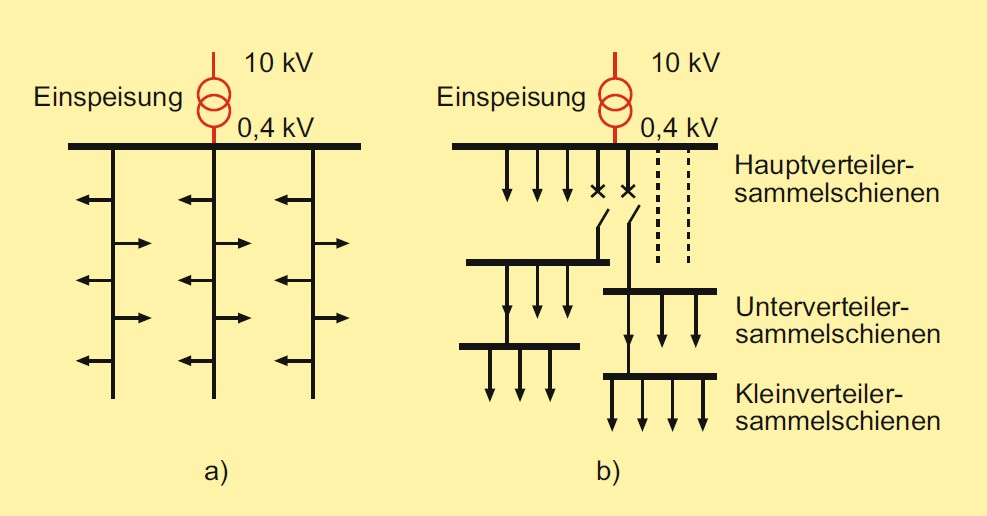
\includegraphics[width=0.98\linewidth]{images/Strahlennetz}
    \caption[Strahlennetz]{Strahlennetz \autocite{Schwab.2012}}
    \label{fig:Strahlennetz}
\end{figure}
\\\\
Bei den Schaltkreisen im Mittelspannungsnetz ist das Management ein wenig komplizierter, da diese für die Hauptversorgung der Niederspannungsschaltfelder 
verantwortlich sind und eine der wichtigsten Knotenpunkte im Stromnetz darstellen. Aus diesem Grund ist es essentiell, diese im Ringnetz oder Maschennetz 
zu versorgen, um auch bei Störungen oder Bauarbeiten eine Versorgungssicherheit zu gewährleisten. Bei einem Ringnetz hängt jede Masche auf zwei Knoten und 
kann somit ähnlich wie beim Maschennetz  in abgewandelter Form von zwei Knoten aus versorgt werden. Änderungen in diesem Netz, \zB durch Baustellen müssen 
immer so geplant werden, dass nur ein Teilstück des Ringes ausgeschaltet wird, um eine Versorgung weiter zu garantieren. Zudem sollte man in den Schaltplänen 
überprüfen, ob es an einer Ust. oder einem Schaltwerk in der Nähe der Baustelle eine offene Verbindung zu einer anderen Masche gibt, um diese ggf. 
dazuzuschalten. Dadurch kommt eine zusätzliche Verbindung im Knoten hinzu, welche bei unerwarteten Störungen größere Stromausfälle vermeiden kann, da der 
Knoten von mehreren Maschen versorgt wird. \autocite{Schwab.2012}
\begin{figure}[hbt]
    \centering
    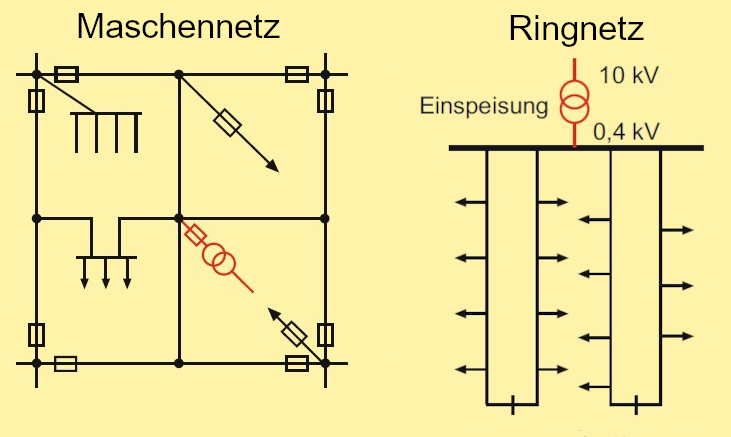
\includegraphics[width=0.98\linewidth]{images/Ring und Maschennetz}
    \caption[Maschen/Ringnetz]{Maschen- und Ringnetz \autocite{Schwab.2012}}
    \label{fig:Maschen/Ringnetz}
\end{figure}
\\\\
Grundsätzlich muss eine Schaltung im Mittelspannungsnetz beim Netzbetreiber des vorgelagerten Netzes  beantragt werden. Dies bedeutet, dass die vorher höher 
gehende Netzebene von einem anderen Netzbetreiber betrieben wird. In diesem Fall betrifft dies den Antrag bei der Netze BW GmbH als Leitstelle. Die Leitstelle 
ist eine Zentrale, in der das komplette Stromnetz der Umgebung überwacht wird und über jegliche Störung informiert wird. Sie ist Informationsempfänger und 
Vermittler für sämtliche Anliegen rund um ihr Einsatzgebiet und ist der erste Ansprechpartner für Mittelspannungsanliegen. Diese überprüfen anschließend ob 
eine Schaltung an den gewünschten Stellen möglich ist und geben diese dann frei. Dieser sogenannte Schaltantrag beinhaltet nicht nur die Genehmigung der 
Schaltung, sondern auch einen genauen Ablauf, wie diese stattzufinden hat. Darunter zählen die Tätigkeiten, des ein- oder ausschalten des Lasttrennschalters, 
wie auch das einlegen oder entfernen der Erde. Die Schaltung des Lasttrennschalters bringt mit sich, ob das angeschlossene Mittelspannungskabel mit der 
Sammelschiene verbunden ist und unter Spannung steht oder nicht. Bei einem ausgeschalteten Kabel, muss der Schalter für die Erde eingelegt werden. Dieser 
funktioniert gleich wie ein Lasttrennschalter, nur das dieser dafür sorgt, dass das Kabel mit der Erde verbunden ist und somit sämtliche Fehlerströme in das 
Erdreich abgeleitet werden. Da dieses Netz im Ring- oder Maschennetz betrieben wird, reicht es nicht aus, den Lasttrennschalter von einer Seite auszuschalten. 
Dieser muss immer auf beiden Enden des Kabels ausgeschaltet werden, um eine Spannungsfreiheit herzustellen. Diese muss anschließend mit einem 
Mittelspannungsprüfer überprüft werden, um sicherzustellen, dass diese auch wirklich vorliegt. Ein Mittelspannungsprüfer ist ein Messgerät zur 
Feststellung der Spannung an Anlagen bis zu einer Nennspannung von 36 kV. Die Messspitze wird hierfür an die Phasen der Sammelschiene gehalten und 
zeigt anschließend an, ob eine Spannung anliegt. \autocite{Pfisterer.}
\\
Nach feststellen der Spannungsfreiheit können nun arbeiten am Kabel oder in der Nähe des Kabels durchgeführt werden. Diese beziehen sich oftmals auf die 
Verlegung neuer Kabel, arbeiten von anderen Bauunternehmen in der Nähe des Kabels oder das Schneiden eines alten oder auszutauschenden Kabels.
\\\\
Das Schneiden eines Mittelspannungskabels funktioniert mit Hilfe einer Sicherheitsschneidanlage. Diese Anlage besteht aus einem hydraulischen Schneidkopf 
und einer zugehörigen Pumpe. Dies bedeutet, dass die gesamte Anlage mit einem nichtleitenden Öl betrieben wird, welches durch erhöhen des Drucks dafür sorgt, 
dass sich der Schneidkopf schließt. Durch Schließen des Schneidkopfes wird das zu schneidende Kabel durchtrennt.
\begin{figure}[hbt]
    \centering
    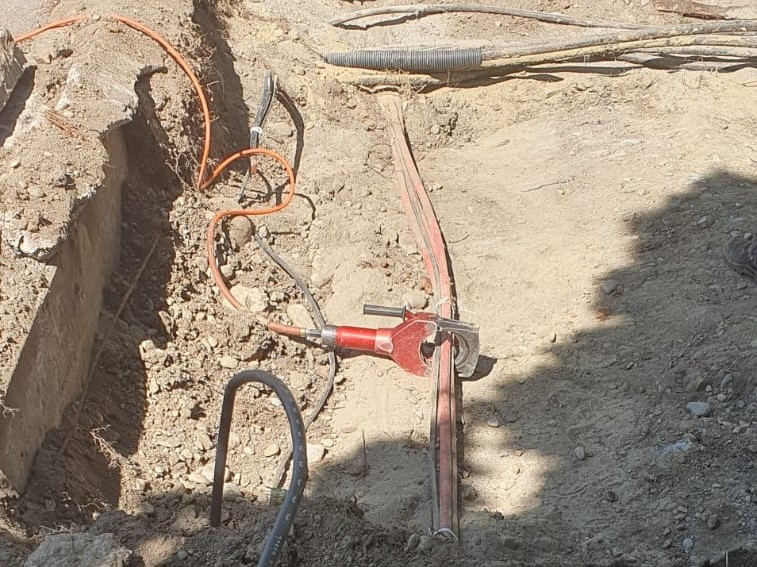
\includegraphics[width=0.98\linewidth]{images/MS_Kabelschnitt.jpeg}
    \caption[MS Schneidung]{Mittelspannungsschneidgerät (eigene Darstellung)}
    \label{fig:MS Schneidgerät}
\end{figure}
\\Im Falle eines unter Spannung stehenden Kabels, sorgt das nichtleitende Öl dafür, dass keine Gefahr für Mitarbeitende entsteht und diese trotzdem das Kabel 
durchtrennen können. Vorausgesetzt wird, dass dieser Fall nicht eintritt. Dafür werden Maßnahmen getroffen, die die Überprüfung der Netzpläne beinhalten, 
um sicherzustellen, dass dieses Kabel inaktiv ist. Zudem muss vor jedem Kabelschnitt Rücksprache mit der zuständigen Leitstelle gehalten werden, welche 
zusätzlich die Spannungsfreiheit und die Zulassung zur Schneidung überprüft und freigibt.  
\clearpage

\section{Schaltfeldmanagement für eine zuverlässige Stromversorgung}

Die Schaltfelder im Niederspannungsnetz haben einen großen Einfluss auf die Effektivität und Funktionalität des Stromnetzes. Um diese Eigenschaften jederzeit 
zu gewährleisten, ist es von Nöten diese Schaltfelder zu überwachen und zu managen. Zudem muss jedes Schaltfeld so zusammengestellt werden, dass selbst bei 
einem unerwarteten Ausfall eine Versorgungssicherheit hergestellt ist. Diese Sicherheit kommt vor allem aus den genannten Punkten der maximalen Nennleistung 
eines Transformators und den verschiedenen Netztypen. Die Nennleistung ist hinsichtlich einer Notsituation von enormer Relevanz, da diese entscheidend ist 
für ein stabiles Netz. Wie im Kapitel 4.2 erläutert, kann ein solcher Transformator auch über kürzere Zeit höhere Leistungen erbringen, welche meist nicht 
von Nöten sind, da die Schaltfelder so aufgeteilt wurden, dass genügend freie Leistung zur Verfügung steht. Sollte ein Transformator an seine Grenzen kommen, 
gibt es die Möglichkeit diesen durch einen größeren auszutauschen oder das Schaltfeld aufzuteilen und eine neue Ust. zu bauen. Nicht nur der Transformator 
sorgt für ein störungsfreies Netz, sondern auch die Selektivität.  Auch der Netztyp, welcher im Kapitel 4.2 vorkommt trägt zu einem stabilen Netz bei. Dies 
liegt vor allem an der Versorgung von zwei oder mehr Seiten, wie es im Ring- oder Maschennetz der Fall ist. Dadurch ist es zusätzlich möglich Baustellen zu 
realisieren, ohne Unterbrechungen im Stromnetz. Das Mittelspannungsnetz ist ein Hauptakteur, wenn es um die Versorgung des Niederspannungsnetzes geht und 
ist Grundvoraussetzung für eine funktionierende Stromversorgung. Dazu hat dies auch den Netztyp des Ring- oder Maschennetzes, um eine Versorgungssicherheit 
zu gewährleisten. Diese Sicherheit kann durch ein Strahlennetz nicht erreicht werden, da es bei einer Störung zu einem Gesamtausfall auf der Länge des 
Strahls kommen würde. Zudem kann in einem Ring- oder Maschennetz flexibel geschaltet werden, um sich den aktuellen Vorkommnissen anzupassen. Die Rücksprache 
und Beantragung von Vorkommnissen im Mittelspannungsnetz mit der Leitstelle tragen zu einer Sicherheit in der Versorgung, als auch beim Mitarbeitenden vor 
Ort bei, da dieser über die Situation informiert ist und sich ggf. schützen kann. Dies erfolgt \zB durch zusätzliche Spannungsprüfungen oder speziellem 
Werkzeug zum schneiden von Kabeln unter Spannung. Dies dient vor allem dazu, vor dem Ernstfall geschützt zu sein, falls eine Fehlinformation durch das 
System übermittelt wurde. Die Problemstellungen im Stromnetz der TWS Netz GmbH wurden durch Anpassungen und Änderungen im Schaltfeld gelöst, um dem 
Verbraucher ein funktionierendes Netz zu gewährleisten. Dazu wurde theoretisches Wissen aus den Theoriephasen angewandt, um eine optimale Entscheidung in 
der Verschaltung zu treffen. 

\clearpage